\indent En esta secci\'on, mostraremos buenos y malos casos para nuestro algoritmo, y a su vez, daremos el tiempo estimado 
seg\'un la complejidad del algoritmo calculada anteriormente.

Como la complejidad presenta dos variables marcadas, como son las capacidades de las mochilas y la cantidad de objetos, decidimos, para obtener datos m\'as concisos, realizar los testeos dejando constante la cantidad de objetos y/o las capacidades.\\

Luego de realizar varios experimentos, llegamos a la conclusi\'on que, dejando constante la cantidad de objetos y trabajando con las capacidades, el mejor caso para nuestro algoritmo es en el cual \textbf{todas las mochilas presentan las mismas capacidades} ya que de esta forma nuestro algoritmo realiza la misma ejecuci\'on para cada una de las mochilas sin repetidos.\\
A continuaci\'on mostraremos un gr\'afico que representa lo enunciado:

\vspace*{0.3cm} \vspace*{0.3cm}
  \begin{center}
 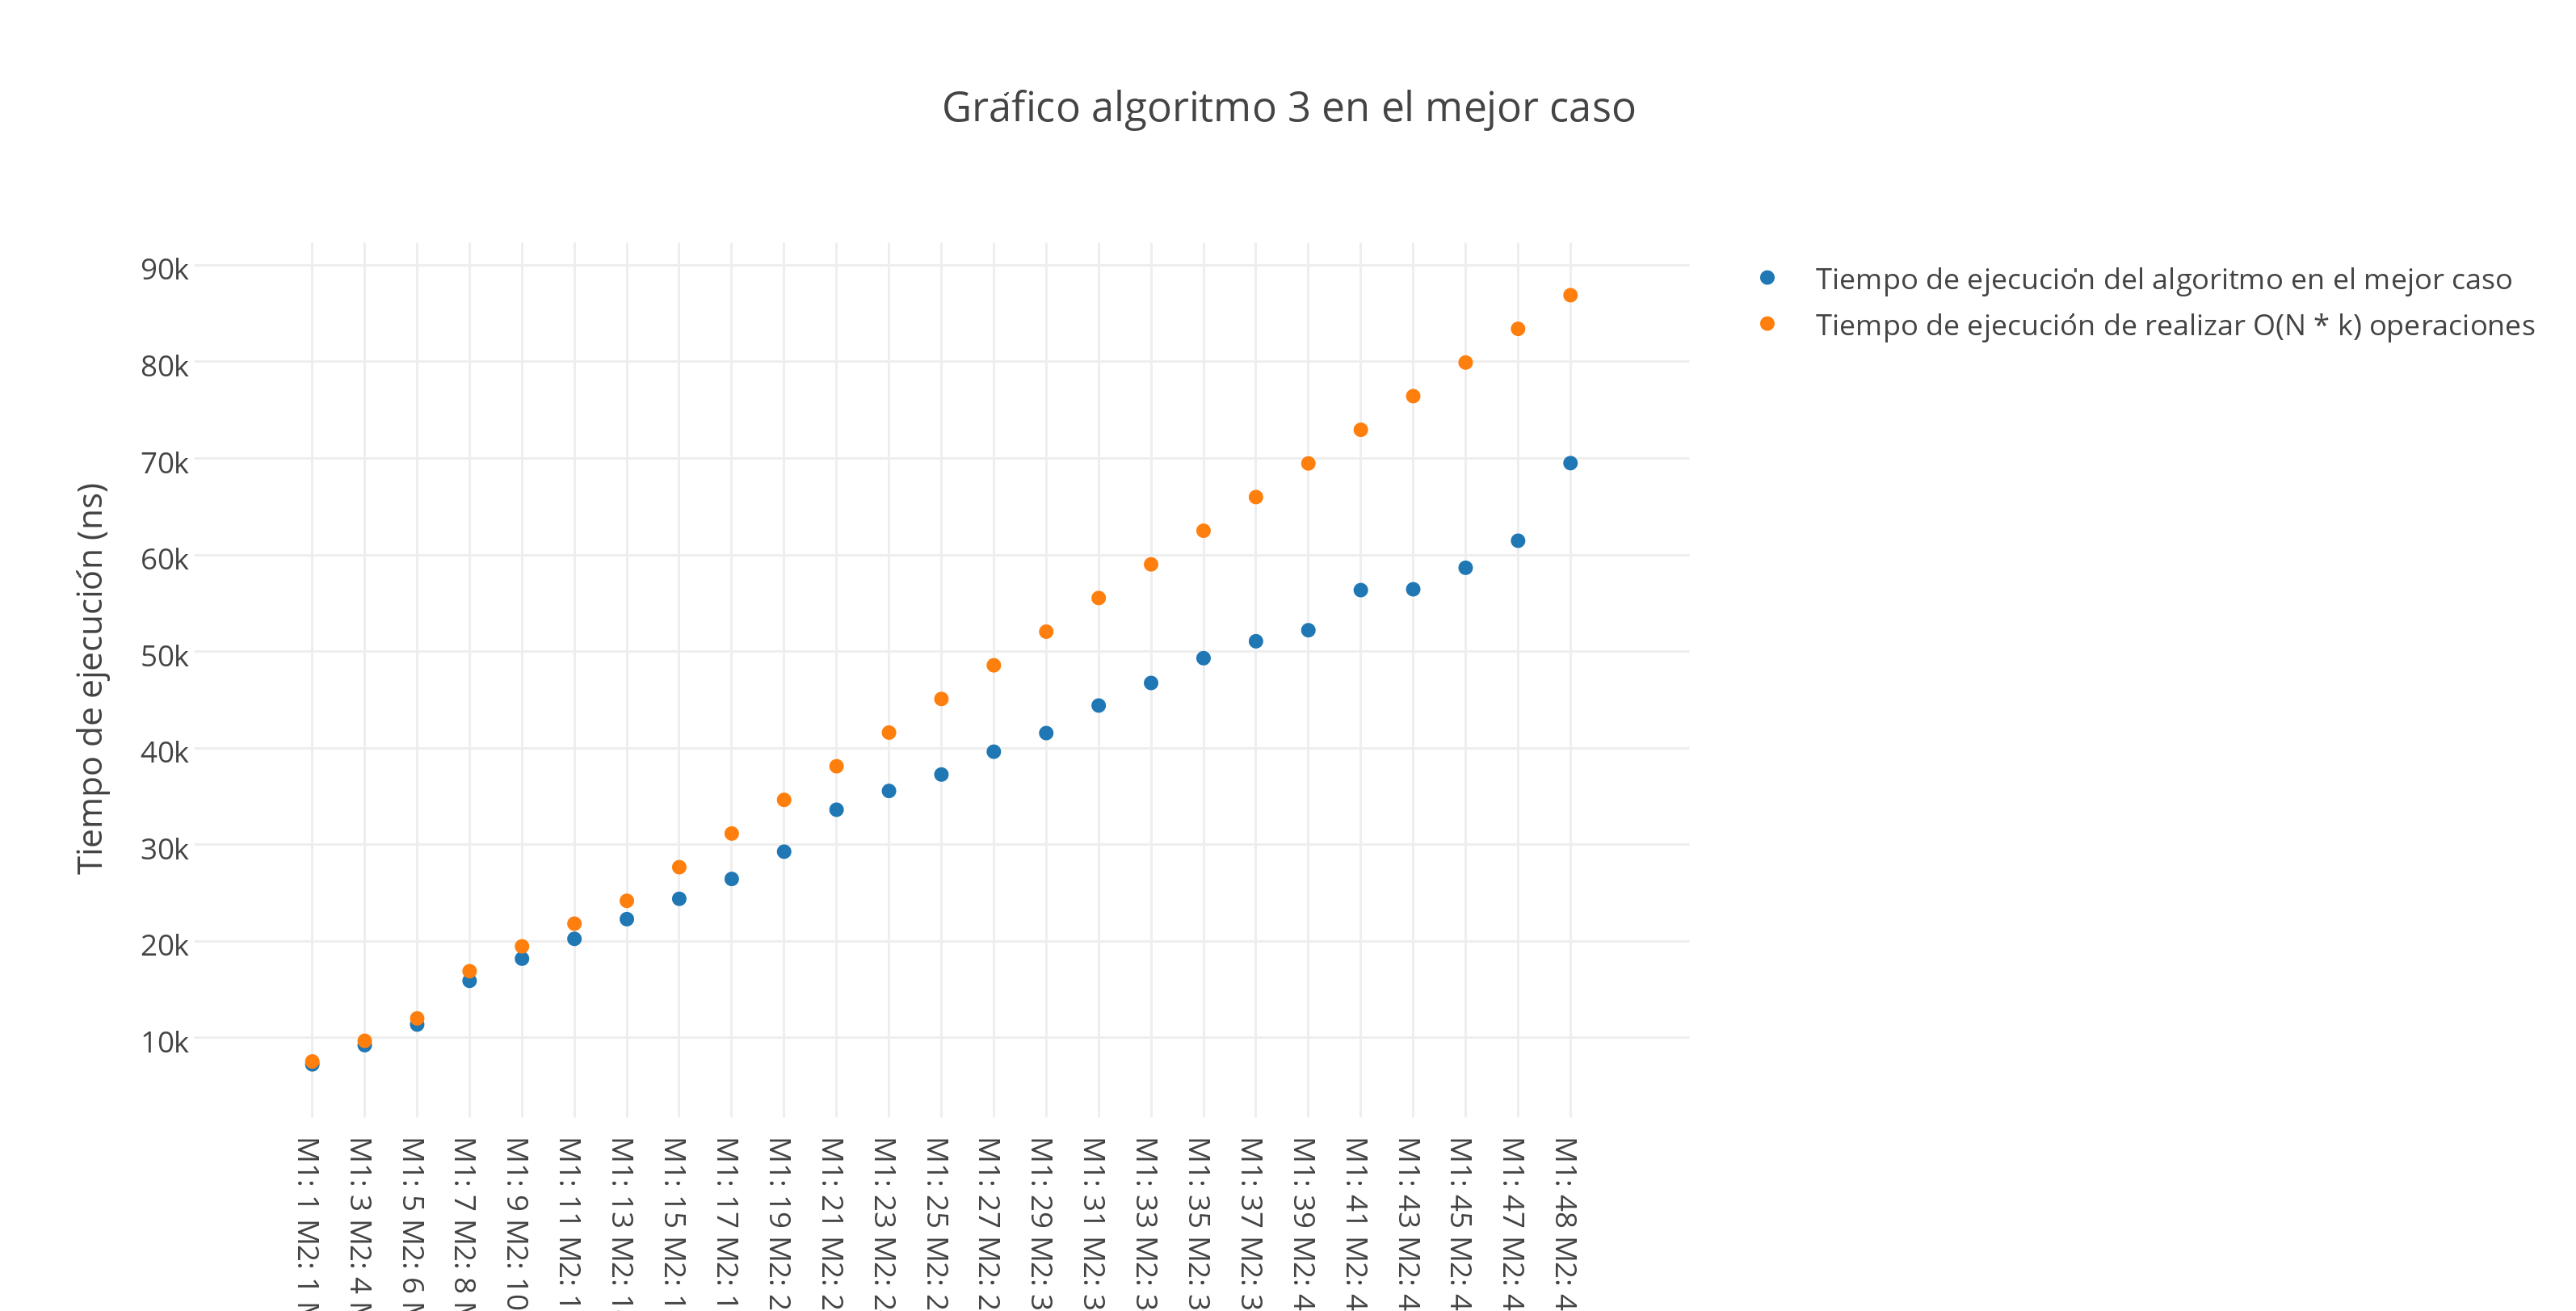
\includegraphics[scale=0.65]{./EJ3/mejorcaso.png}
 {$Gr$\'a$fico$ \ 3.1 - $Mejor$ $caso$ $del$ $algoritmo$}
  \end{center}
  \vspace*{0.3cm}

Dividiendo por la complejidad calculada se obtuvo lo siguiente:\\

\vspace*{0.3cm} \vspace*{0.3cm}
  \begin{center}
 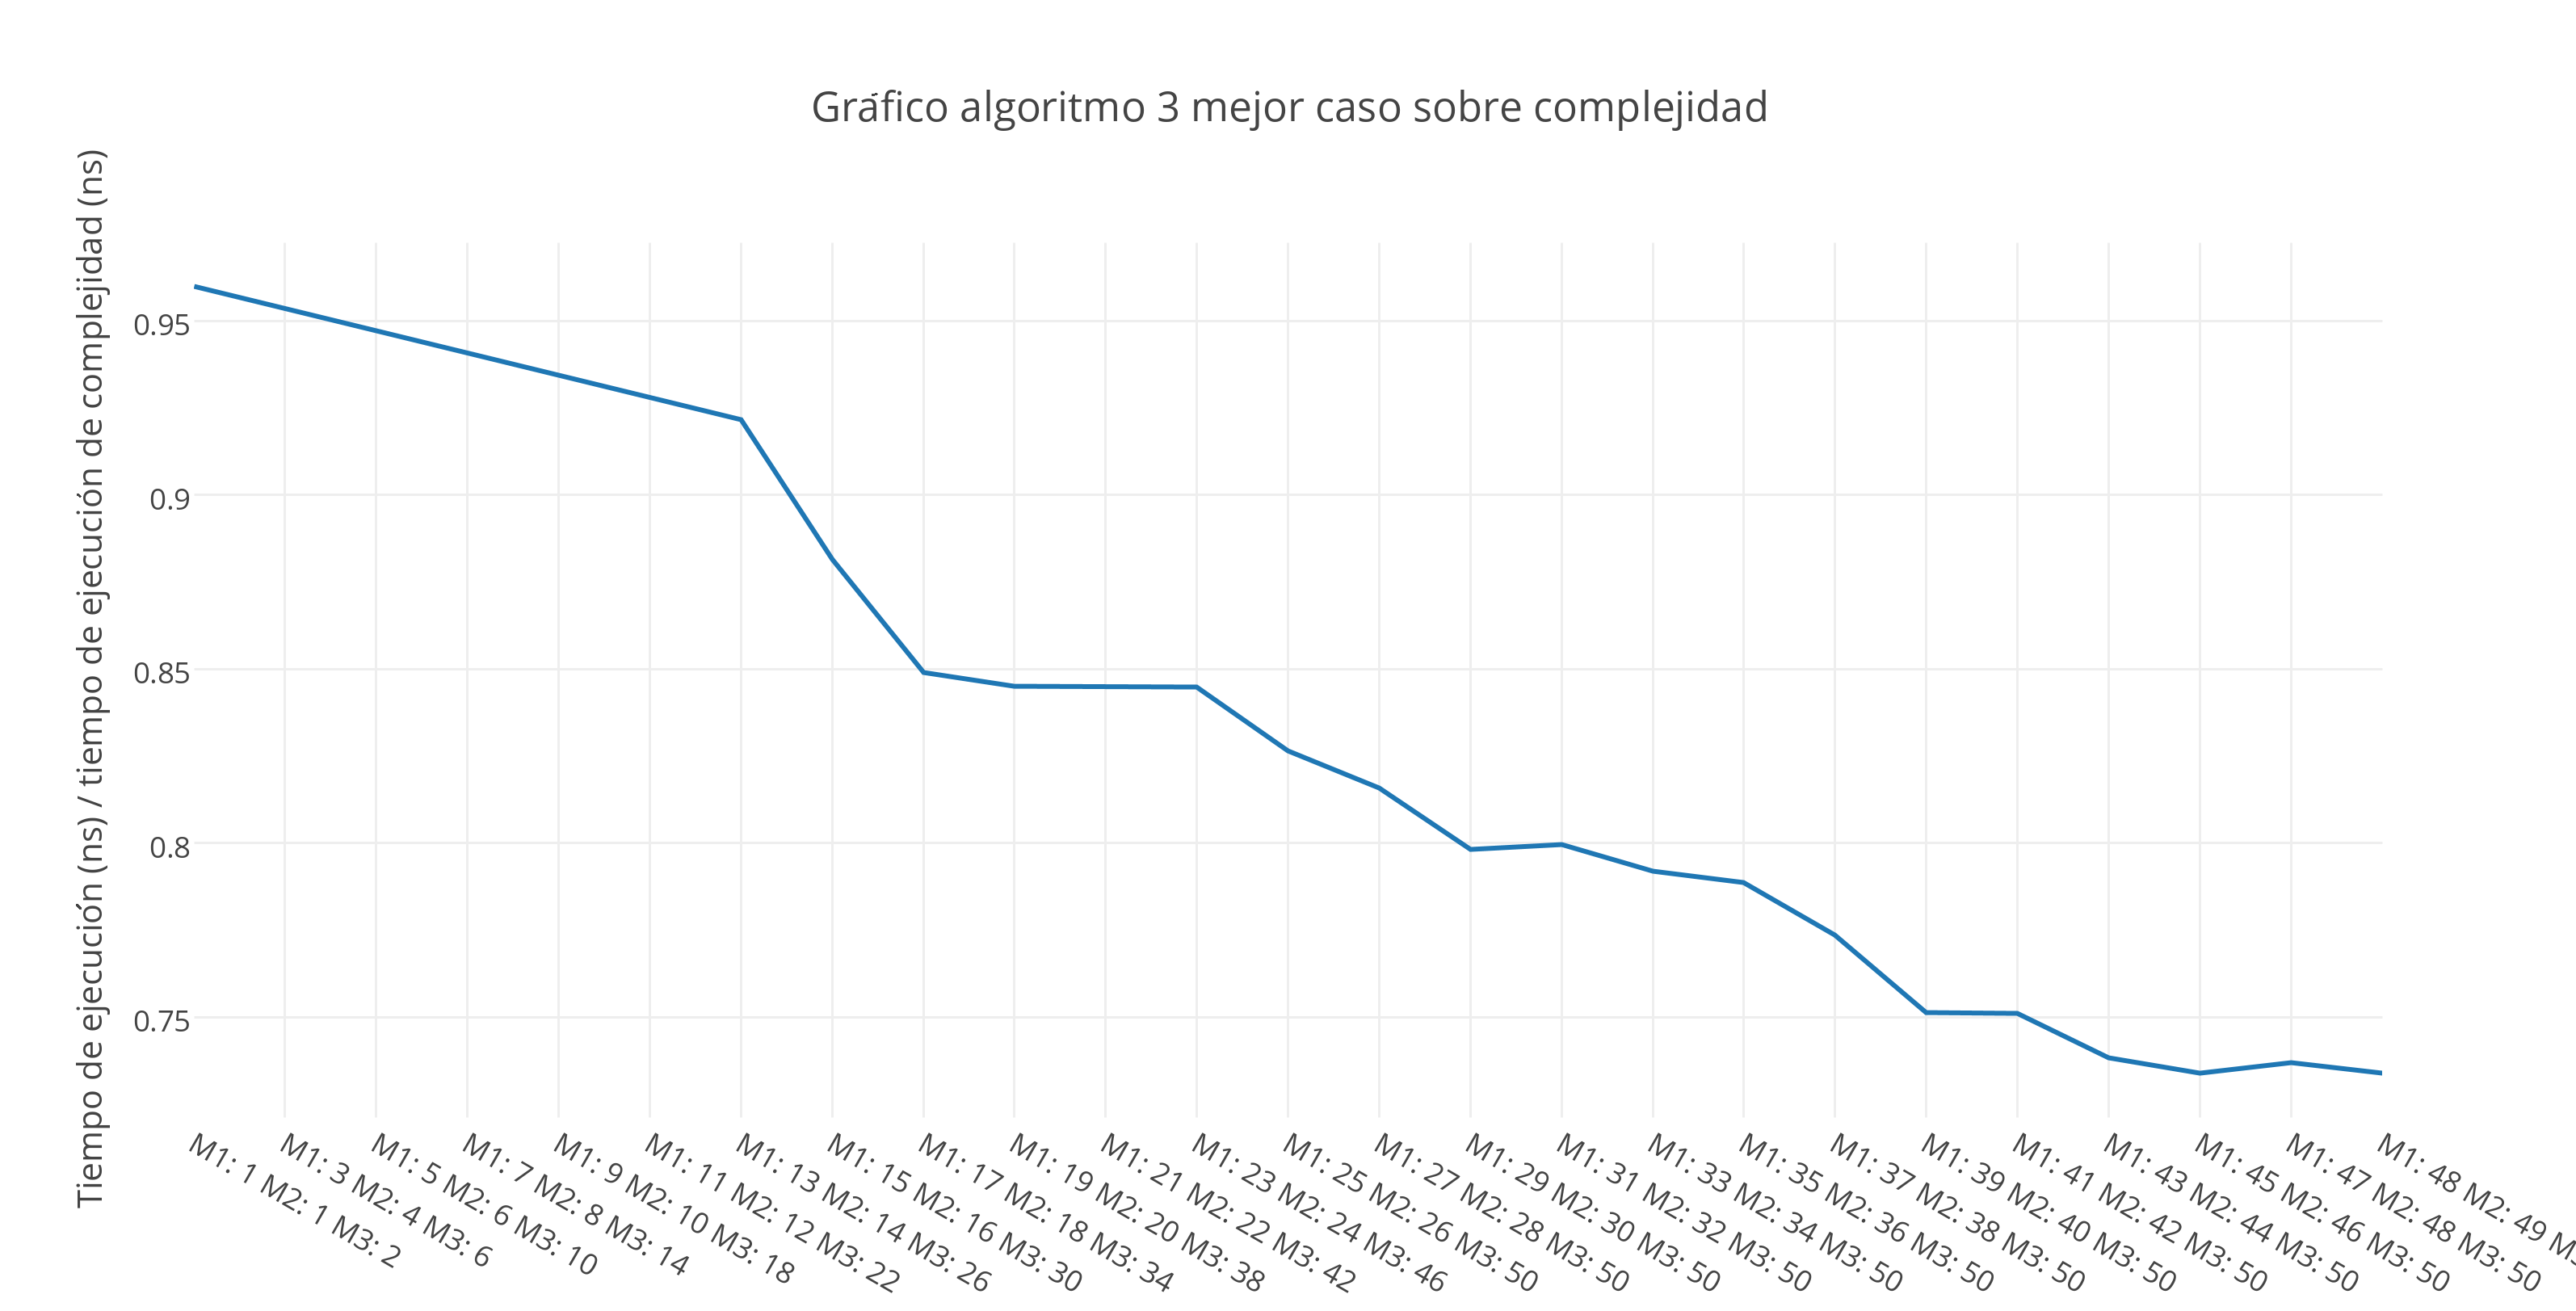
\includegraphics[scale=0.65]{./EJ3/mejorcaso1.png}
 {$Gr$\'a$fico$ \ 3.2 - $Mejor$ $caso$ $del$ $algoritmo$ $sobre$ $complejidad$}
  \end{center}
  \vspace*{0.3cm}
  
Se puede ver en el gr\'afico 3.1 que, dado nuestro algoritmo, al tener las capacidades iguales, el mismo realizar\'a la optimizaci\'on de 3 matrices que simbolizan a cada mochila por separado, lo que nos dar\'a una complejidad acotada por la capacidad de las mochilas por la cantidad de elementos que en esta evaluaci\'on es constante, simplificando lo dicho nos quedar\'ia O($K_{1}\ast N$) + O($K_{2}\ast N$) + O($K_{3}\ast N$) y como $K_{1} = K_{2} = K_{3}$ nos queda que la complejidad para el mejor caso esta acotada por O($K \ast N$) con N constante.\\
Luego, en el gr\'afico 3.2, en el cual dividimos el tiempo de ejecuci\'on de dicho caso con el tiempo de realizar O(N $\ast$ k) operaciones nos da una funci\'on resultante la cual se encuentra por debajo de 1 y tiende a 0 cuando la entrada aumenta corroborando lo que acabamos de decir.\\

Manteniendo el mismo razonamiento, el peor caso para nuestro algoritmo se da cuando hay \textbf{mochilas con capacidades distintas} ya que el algoritmo deber\'a decidir en que mochila colocar el objeto para que el resultado sea \'optimo. Por consiguiente, mostraremos un gr\'afico que representa lo hablado:\\

\vspace*{0.3cm} \vspace*{0.3cm}
  \begin{center}
 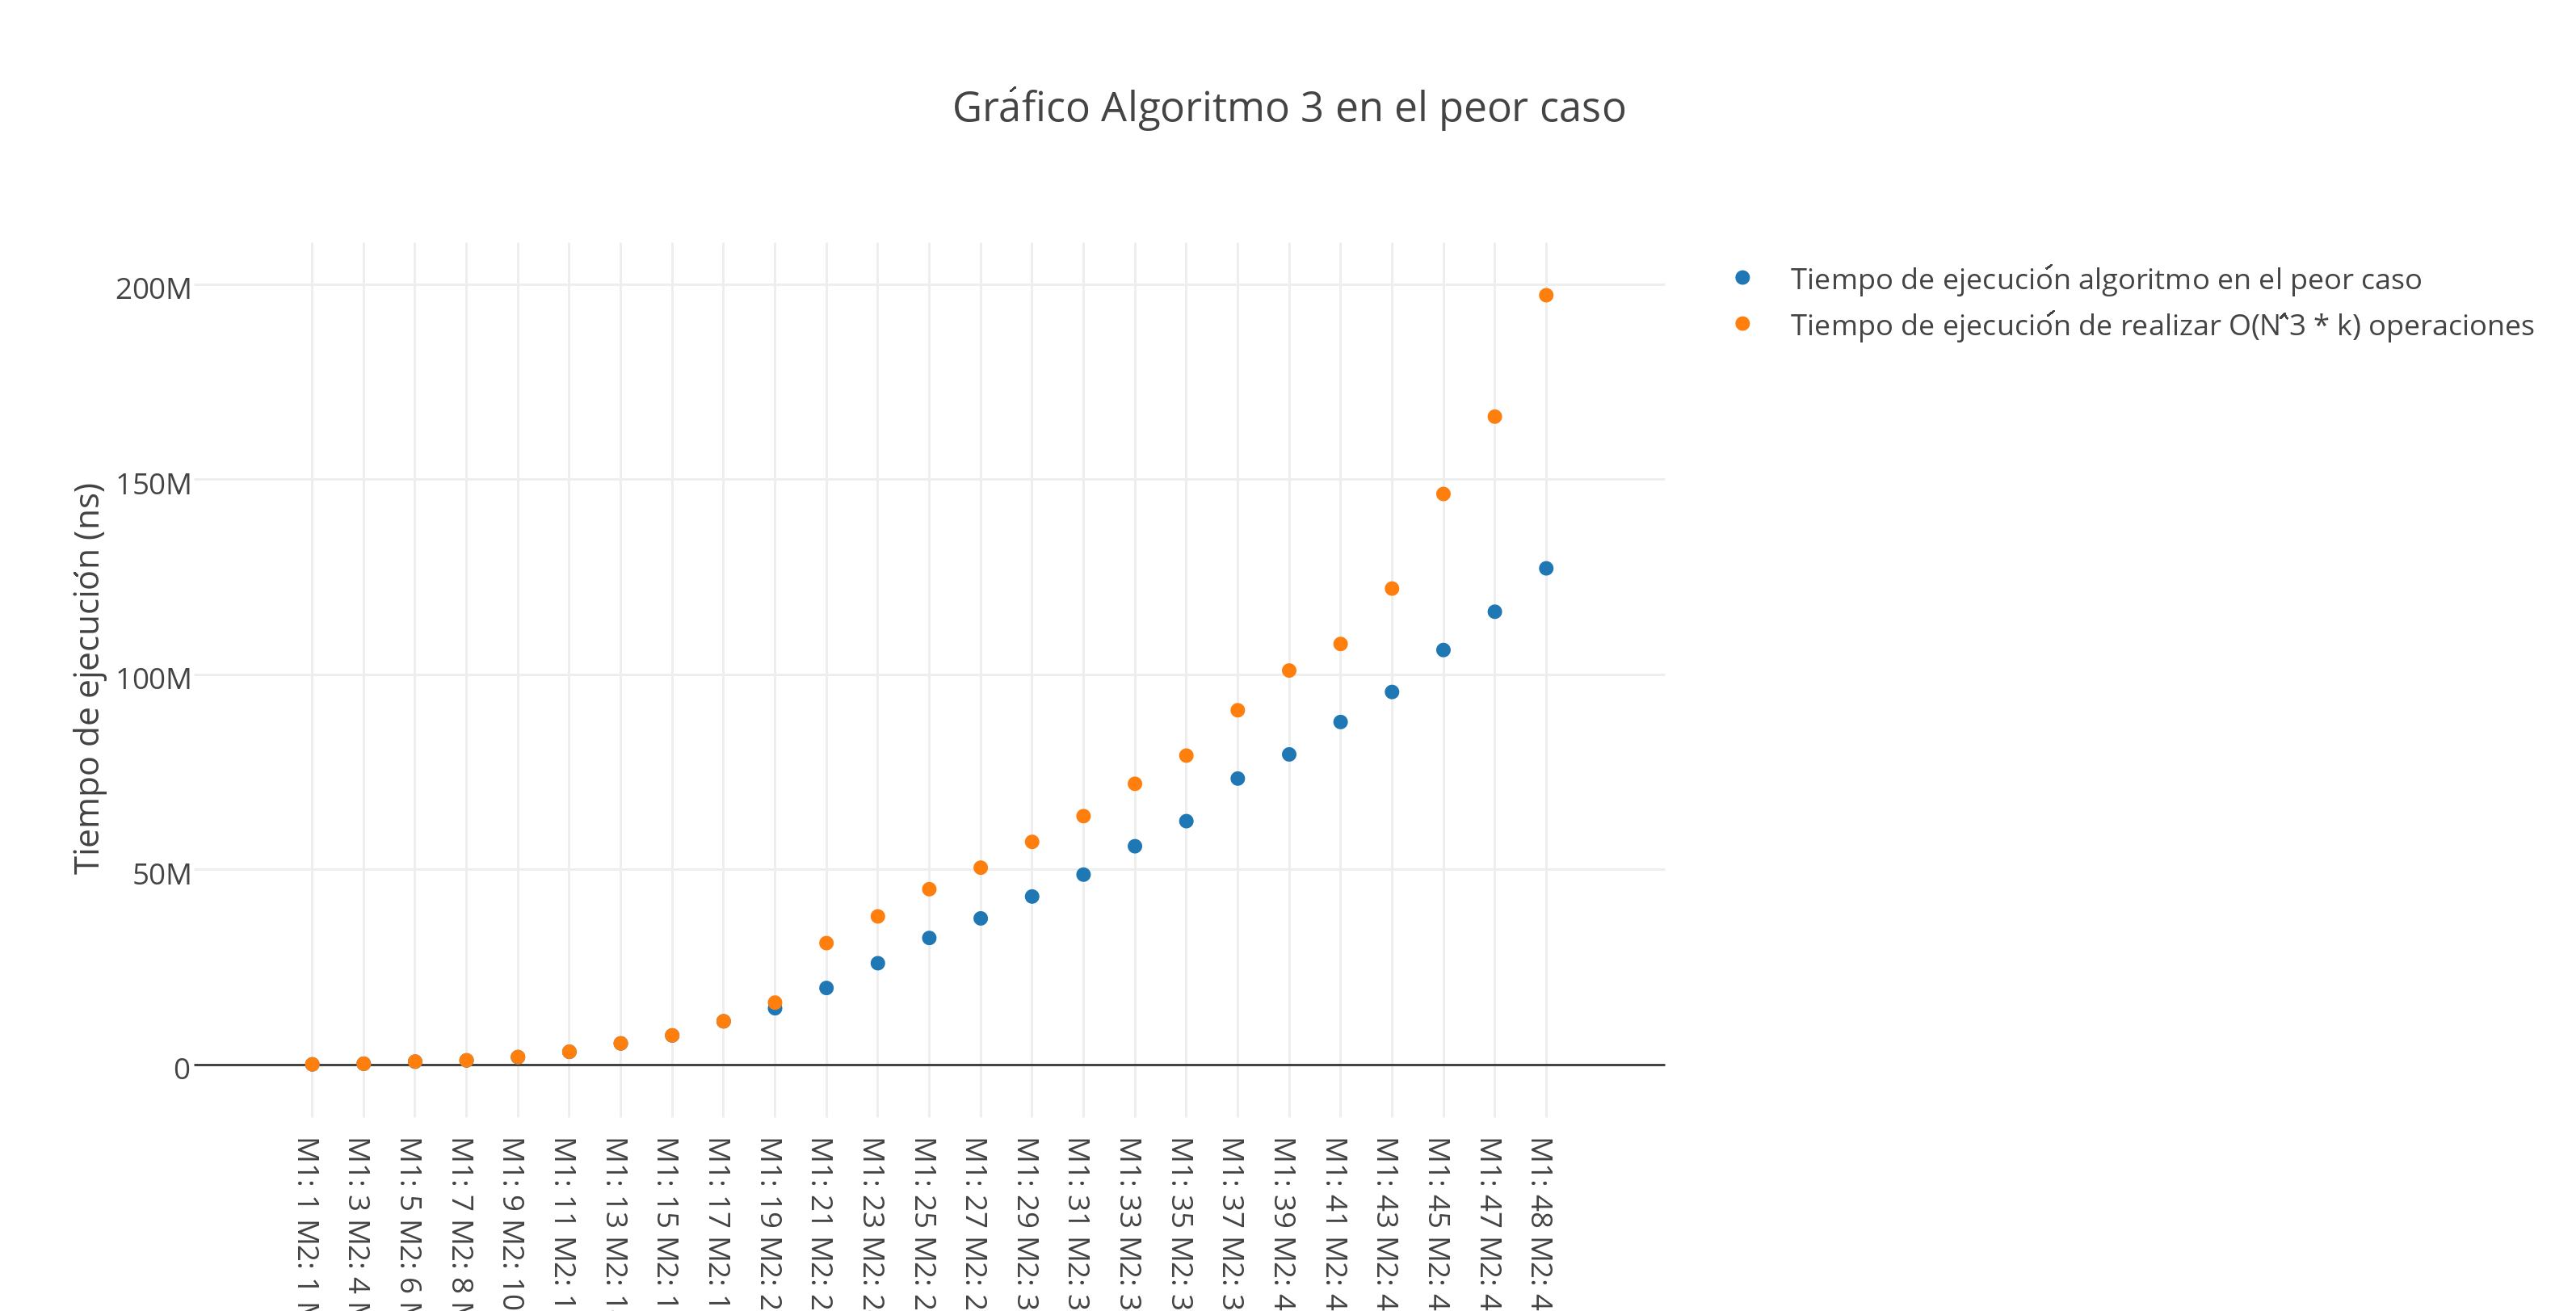
\includegraphics[scale=0.65]{./EJ3/peorcaso.png}
 {$Gr$\'a$fico$ \ 3.3 - $Peor$ $caso$ $del$ $algoritmo$}
  \end{center}
  \vspace*{0.3cm}

Dividiendo por la complejidad calculada se obtuvo lo siguiente:\\

\vspace*{0.3cm} \vspace*{0.3cm}
  \begin{center}
 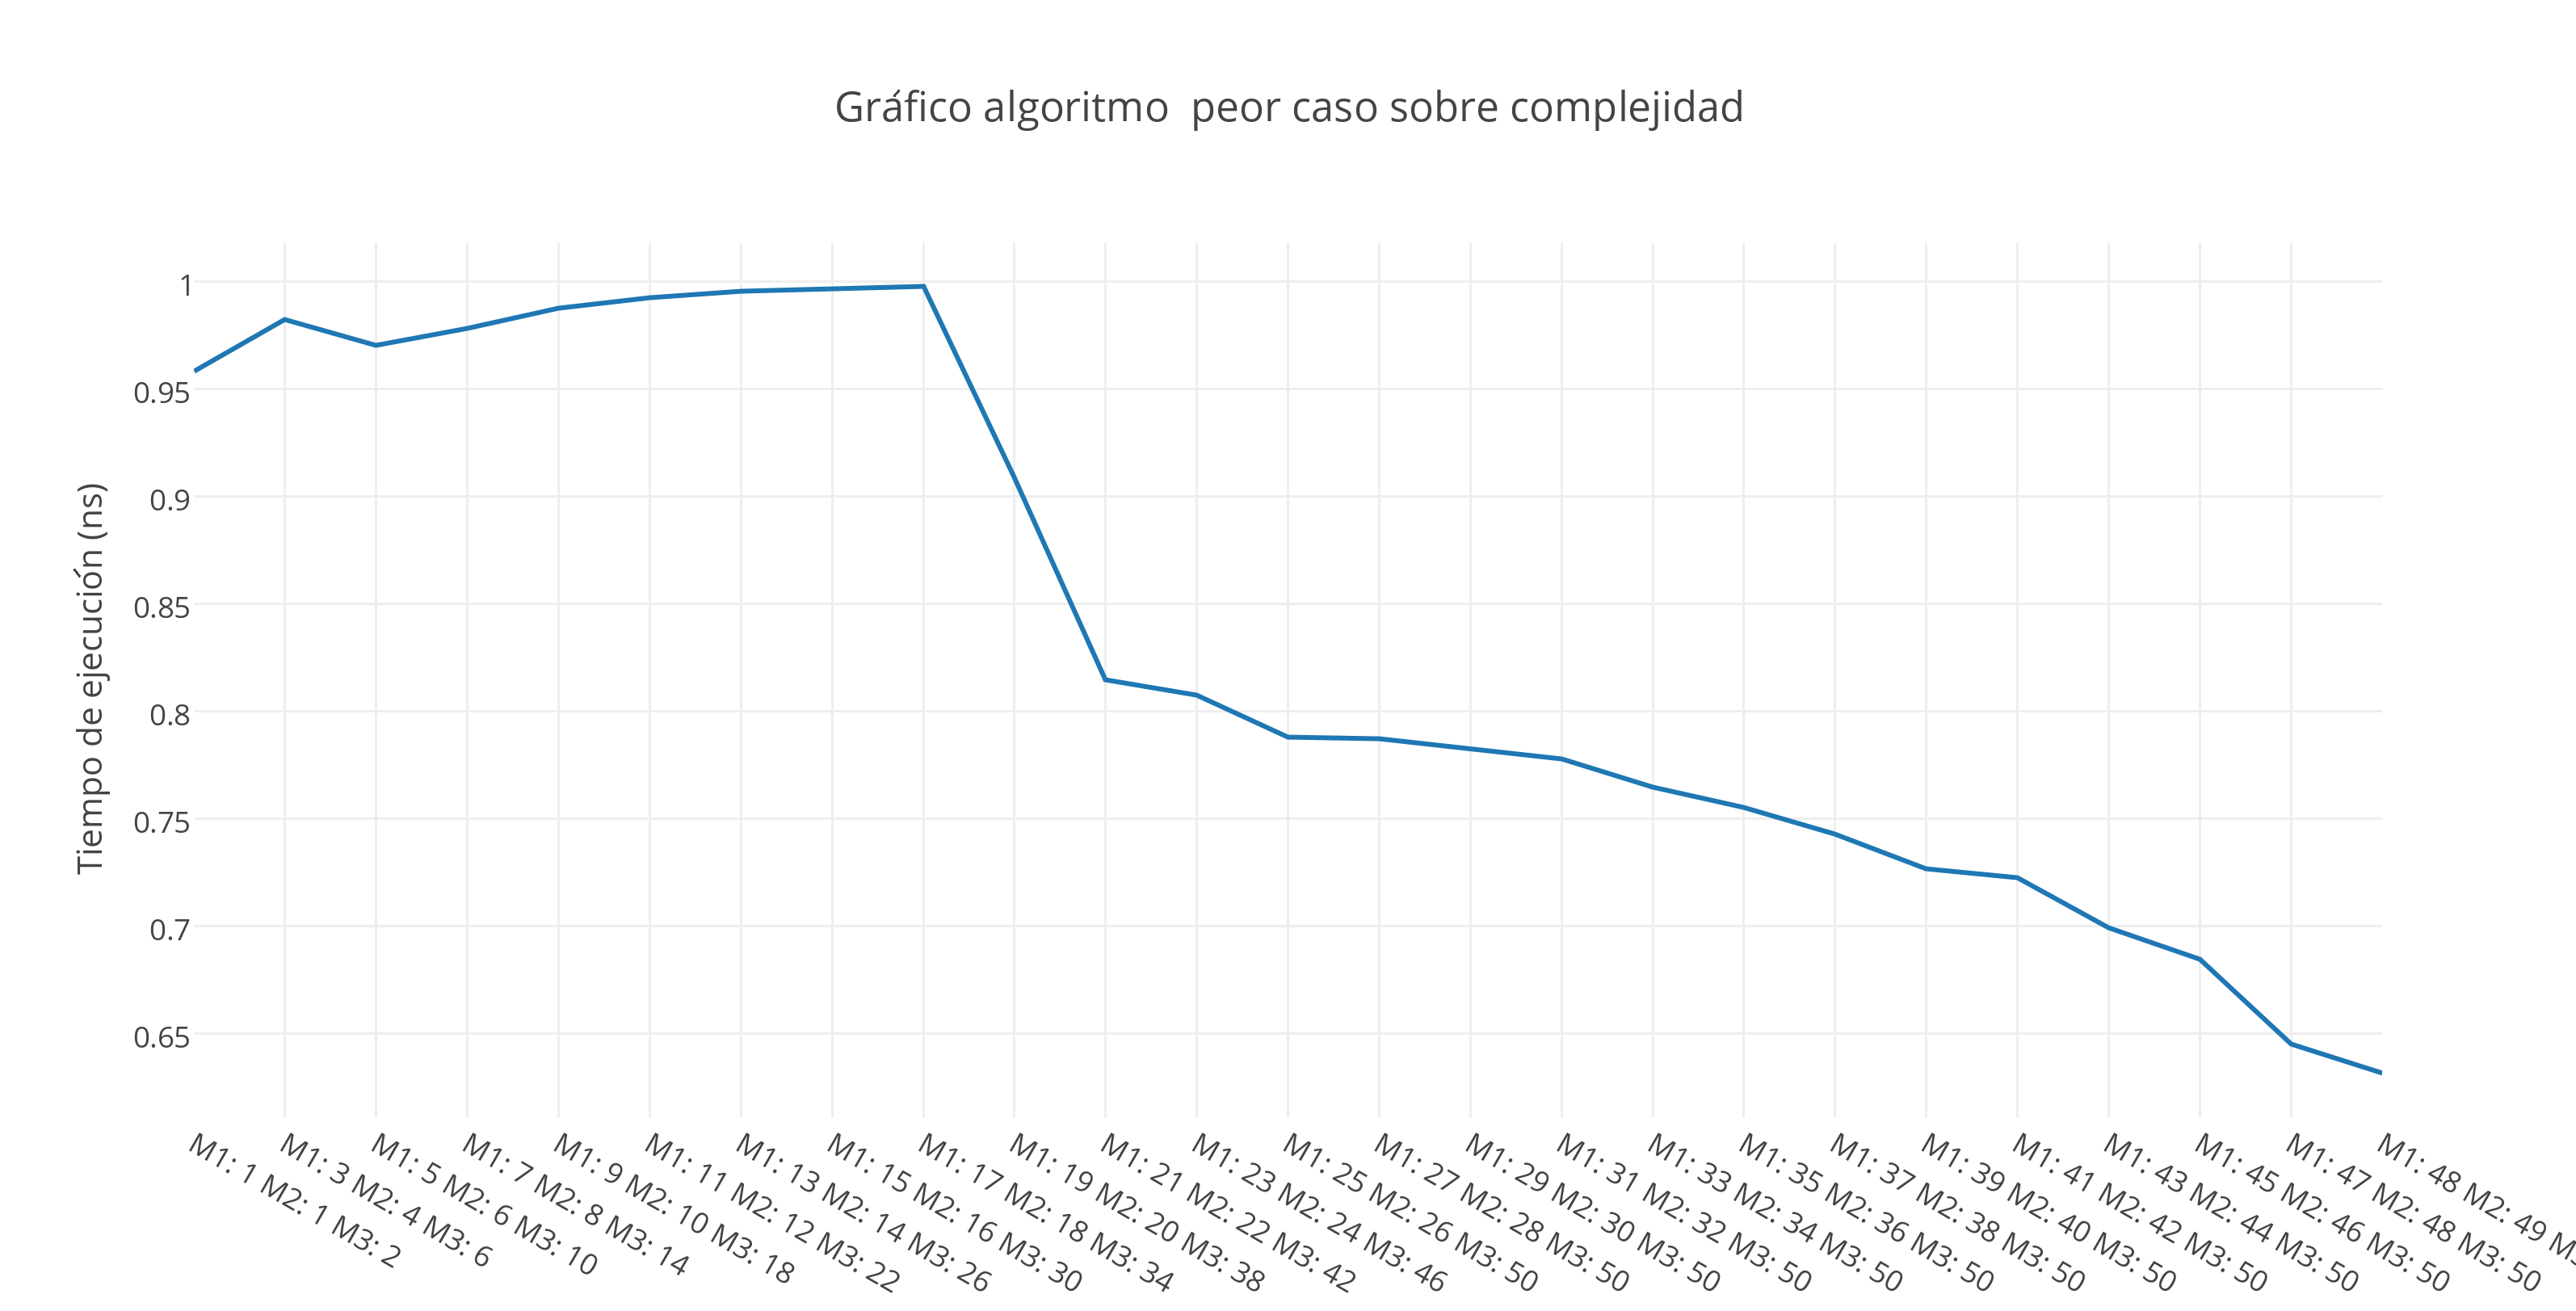
\includegraphics[scale=0.65]{./EJ3/peorcaso1.png}
 {$Gr$\'a$fico$ \ 3.4 - $Peor$ $caso$ $del$ $algoritmo$ $sobre$ $complejidad$}
  \end{center}
  \vspace*{0.3cm}
  
  
Es posible observar en el gr\'afico 3.3 que, dado nuestro algoritmo, al tener las capacidades distintas, el mismo realizar\'a la optimizaci\'on de 3 matrices que simbolizan a cada mochila anidadas, lo que nos dar\'a una complejidad acotada por la capacidad de las mochilas al cubo por la cantidad de elementos que en esta evaluaci\'on es constante, simplificando lo dicho nos quedar\'ia O($(K_{1}\ast K_{2} \ast K_{3}) \ast N$) nos termina quedando que la complejidad para el peor caso esta acotada por O($K^{3} \ast N$) con N constante.\\
Luego, en el gr\'afico 3.4, en el cual dividimos el tiempo de ejecuci\'on de dicho caso con el tiempo de realizar O($K^{3} \ast N$) operaciones nos devuelve una funci\'on resultante la cual se encuentra por debajo de 1 y tiende a 0 cuando la entrada aumenta corroborando lo que acabamos de decir.\\

Por finalizado, es notorio que, tanto en el gr\'afico 3.2 como 3.4 la funciones resultantes siempre se mantienen por debajo de 1, con lo cual se ve que tanto en el mejor como en el peor caso nuestro algoritmo sigue estando acotado por la complejidad calculada.\\

Luego, como nuestro algoritmo calcula lo mismo para cualquier tipo de objeto, ya sean todos iguales o no, todos ser\'an casos promedios, salvo el caso en el cual no haya ning\'un tipo de objeto que entre en alguna mochila, este caso podr\'iamos tomarlo como \'el mejor ya que nuestro algoritmo corta al ver que no puede colocar ning\'un objeto dentro de alguna mochila.\\
Dejando de lado este caso, el resto de los mismos tendr\'an un tiempo de ejecuci\'on similar.\\

Mostraremos en el siguiente gr\'afico de ejemplo lo hablado recientemente:\\

\vspace*{0.3cm} \vspace*{0.3cm}
  \begin{center}
 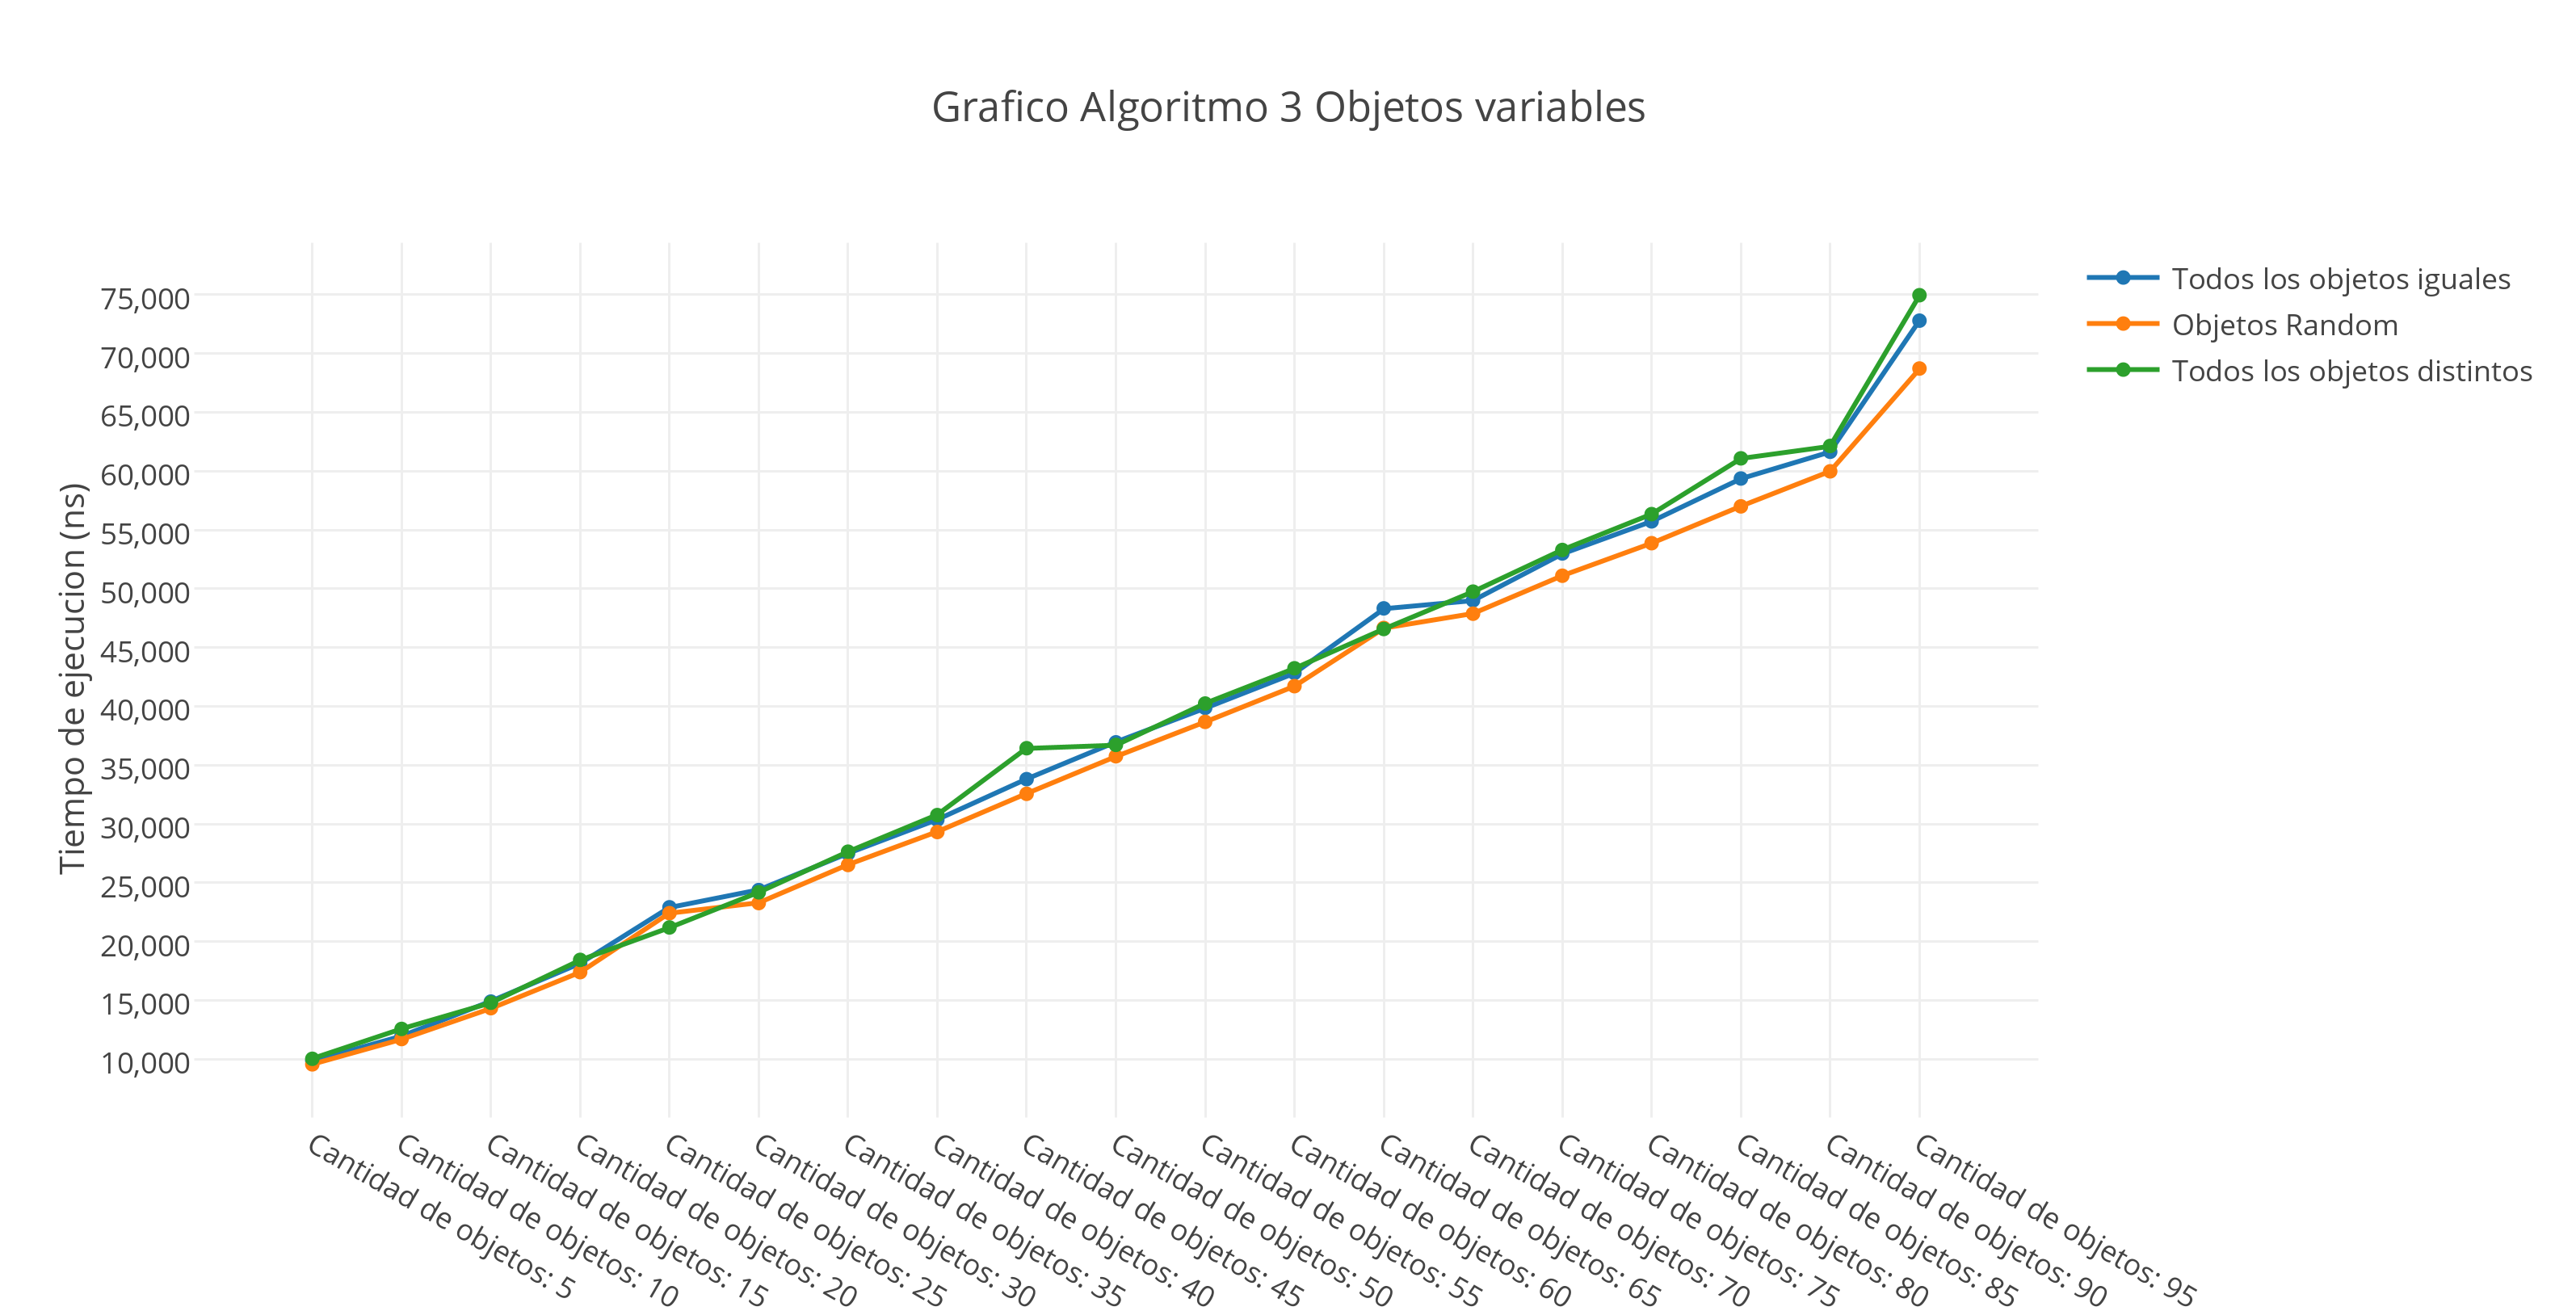
\includegraphics[scale=0.65]{./EJ3/objetos.png}
  {$Gr$\'a$fico$ \ 3.5 - $Objetos$ $Variables$ $y$ $Capacidades$ $Constantes$}
  \end{center}
  \vspace*{0.3cm}
  
Se puede ver en el gr\'afico 3.5 como las 3 funciones, las cuales simbolizan el tiempo de ejecuci\'on del algoritmo con todos los objetos iguales, todos distintos y random, presentan un tiempo de ejecuci\'on similar, como hab\'iamos comentado anteriormente esto se da ya que nuestro algoritmo realiza las mismas operaciones para cualquier tipo de objeto en las que chequea si es \'optimo o no agregar un elemento a alguna mochila.\\

Trabajando con los objetos variables y habiendo dejado constante la capacidad de las mochilas se llega a que la complejidad esta acotada por la cantidad de elementos multiplicada por la capacidad de las mochilas, en este caso constante para las 3 e igual a 20 en todas las corridas y entradas.\\

Luego, podemos concluir que por lo visto en los gr\'aficos se puede afirmar que nuestro algoritmo esta acotado por la complejidad solicitada anteriormente.\\